\documentclass[tikz,border=2pt]{standalone}
\usepackage{amsmath,amssymb}
\usepackage{tikz}

\begin{document}
% x1 + x2 <= 100 + 50y: without the new machine (y = 0) production stays in the small
% triangle; buying it (y = 1) adds the band up to 150.
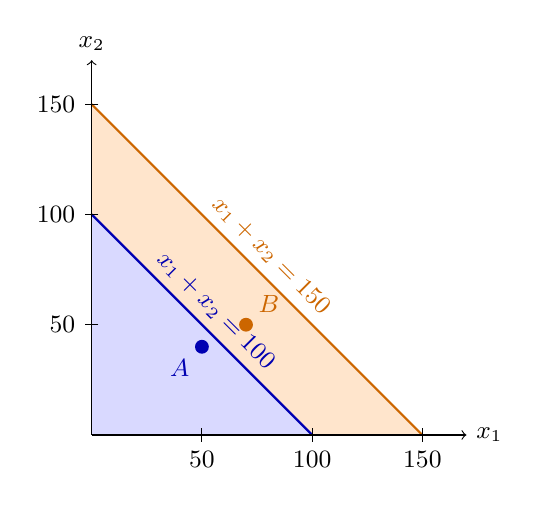
\begin{tikzpicture}[every node/.style={font=\small}, x=0.028cm, y=0.028cm]
	\fill[orange!20] (0,100) -- (100,0) -- (150,0) -- (0,150) -- cycle;
	\fill[blue!15] (0,0) -- (100,0) -- (0,100) -- cycle;
	\draw[blue!70!black, thick] (100,0) -- (0,100) node[pos=0.5, above, sloped, font=\small] {$x_1+x_2=100$};
	\draw[orange!80!black, thick] (150,0) -- (0,150) node[pos=0.5, above, sloped, font=\small] {$x_1+x_2=150$};
	\draw[->] (0,0) -- (170,0) node[right, font=\small] {$x_1$};
	\draw[->] (0,0) -- (0,170) node[above, font=\small] {$x_2$};
	\foreach \x in {50,100,150} {\draw (\x,3) -- (\x,-3) node[below, font=\small] {$\x$};}
	\foreach \y in {50,100,150} {\draw (3,\y) -- (-3,\y) node[left, font=\small] {$\y$};}
	\fill[blue!70!black] (50,40) circle (2.5pt); \node[blue!70!black, font=\small, below left=1pt] at (50,40) {$A$};
	\fill[orange!80!black] (70,50) circle (2.5pt); \node[orange!80!black, font=\small, above right=1pt] at (70,50) {$B$};
	\end{tikzpicture}
\end{document}
